\chapter{ROW}

\section{概述}

想象有一日志系统(CDP),快照就是日志系统里的时间点。
当前卷的状态依赖于前面的日志记录。

ROW与此类似,删除快照实现复杂,同时需要优化读性能。

ROW设计问题
\begin{enumbox}
\item 链式快照和树状快照
\item 平安需求:可写快照?
\item ***
\item 卷和快照的关系,是共存于一个物理卷、还是各自独立构成一个物理卷。若独立占有一个物理卷,则打快照后,会改变卷ID,凡是依赖于这个信息的地方都需要进行适配。
\item 在哪一层实现ROW
\item 索引的page cache
\item 跨卷读,clone
\item 读取需要合并多个快照上的数据块。建立全量索引及其cache可以加速这一过程。
\item 快照头的映射表如何组织?是全索引,还是增量索引?
\item ROW读快照和读卷是同一个过程?
%\item COW里卷上有完整数据,快照有增量数据。
%\item ROW第一次快照有全量数据,后续快照和卷无完整数据。ROW很自然地体现了增量过程。
\end{enumbox}

\section{操作}

\subsection{create}

\begin{center}
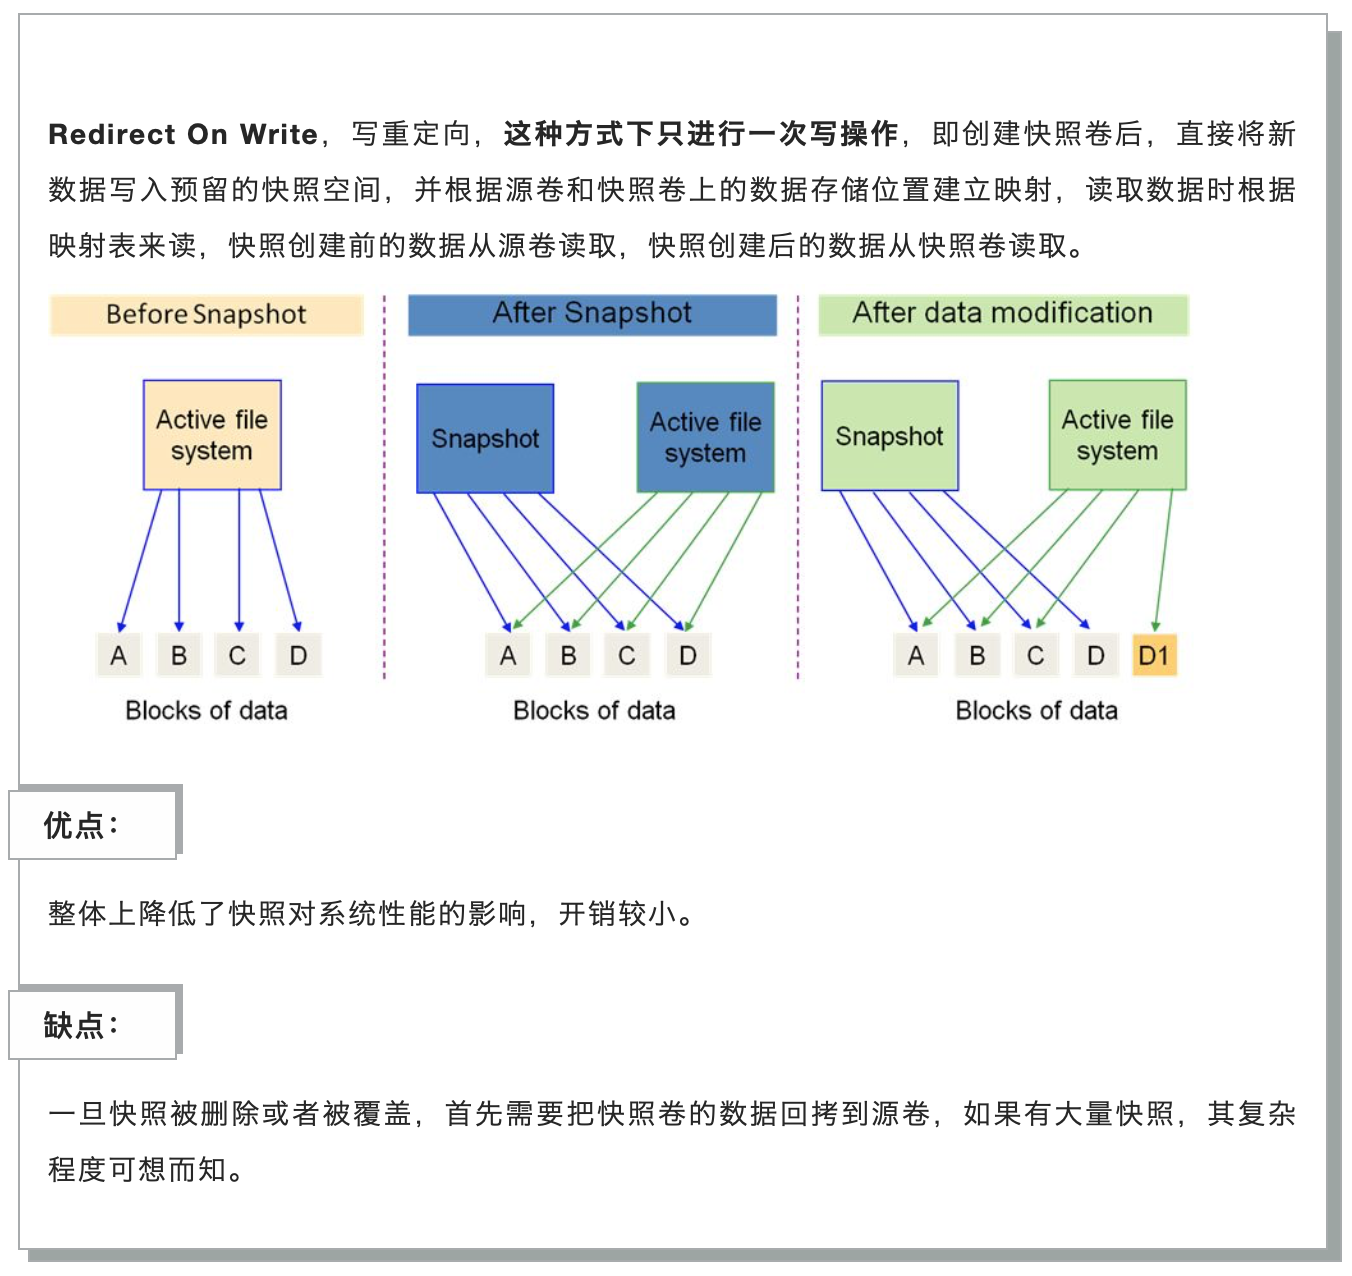
\includegraphics[height=10cm]{../imgs/snapshot/row-snapshot.png}
\end{center}

如果发生卷ID变化,上层应用需要重新打开卷,影响较大。

用户通过命令行创建快照,卷的描述符应有快照方面的信息。

创建快照是通过哪个leader执行的?

从leader方面看,client端与rangectl都需要快照树的结构信息,怎么在多个节点之间进行同步?
加入version,每个holder维护该属性,消息中也携带该属性,如果发现过期,则做相应处理。

如果有多个client端,如何一一通知到呢?

\subsection{delete}

\begin{center}
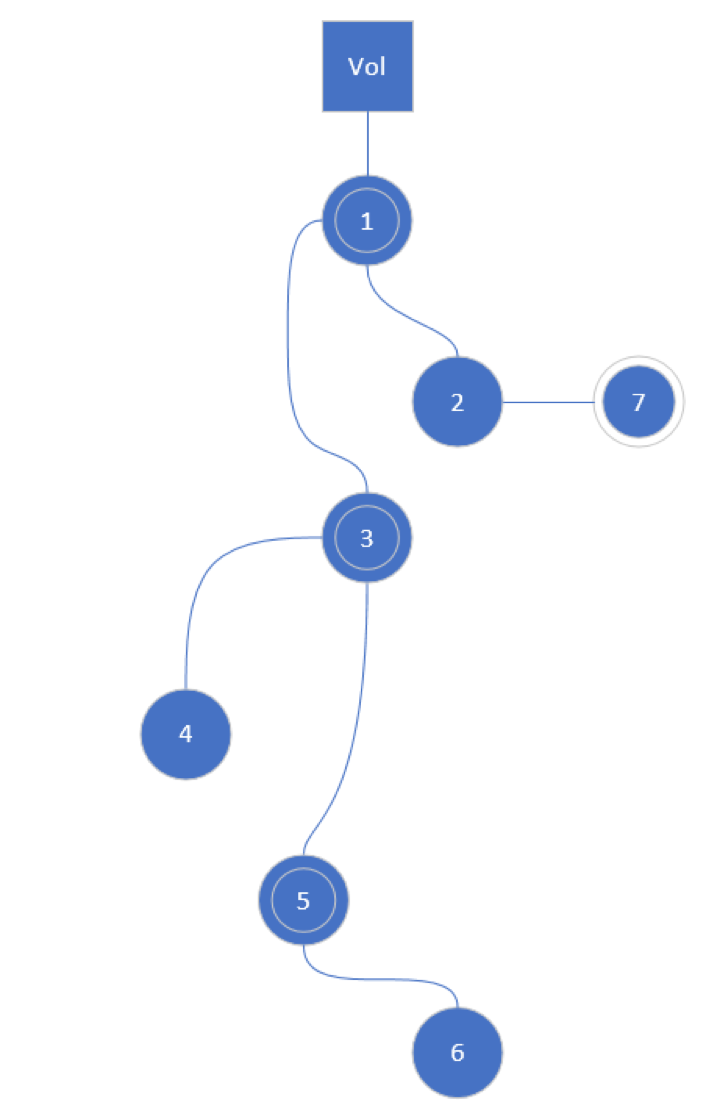
\includegraphics[height=10cm]{../imgs/snapshot/snaptree.png}
\end{center}

快照包含有增量数据,除了叶子快照,不能直接删除。
\begin{enumbox}
\item 根节点,不可删除,只有当快照节点仅剩本节点,并且发生回滚时删除,卷回到无快照状态
\item 快照中间节点
\item 快照中间节点
\item 快照叶子节点
\item 快照中间节点
\item 快照叶子节点
\item 卷所在位置,随着回滚在各个快照上漂移。
\end{enumbox}

空间回收策略
\begin{enumbox}
\item 叶子节点删除,可以完全回收在该时刻之后分配的空间
\item 中间节点,比如3,删除后其实还存在,当子节点删除后自动删除,因此在真正删除前并不能回收空间;
\item \hl{同时,当1上没有其他子节点时,可以做向上合并}。
\end{enumbox}

\begin{center}
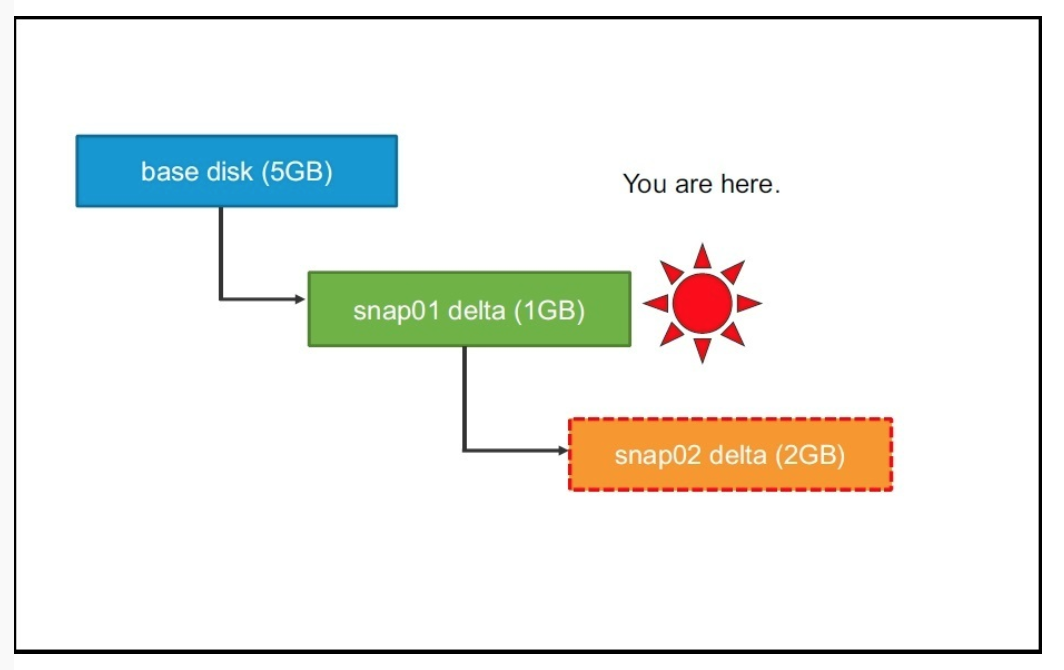
\includegraphics[width=10cm]{../imgs/snapshot/snap-delete-leaf.png}
\end{center}

\begin{center}
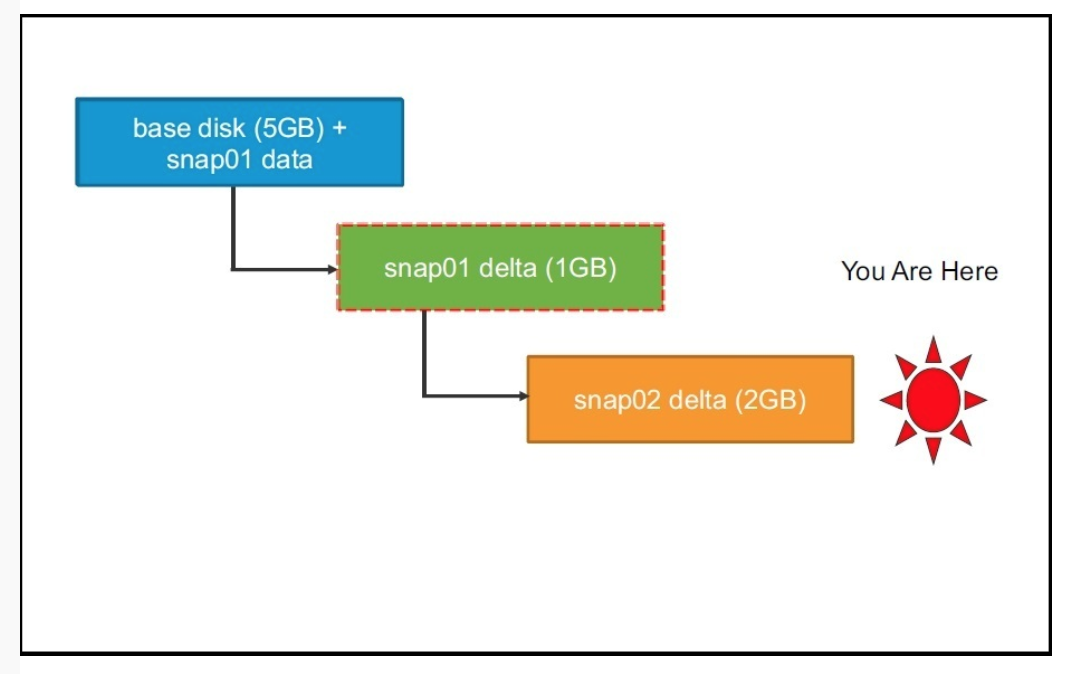
\includegraphics[width=10cm]{../imgs/snapshot/snap-delete-non-leaf.png}
\end{center}


\subsection{rollback}

直接用目标快照的快照头替换卷的快照头。

回收卷私有数据

\subsection{list}

快照树,隐藏或显示删除的快照。

\subsection{read}

\subsection{clone}

读取snapshot的内容。读取卷和快照是同一个过程。

\begin{center}
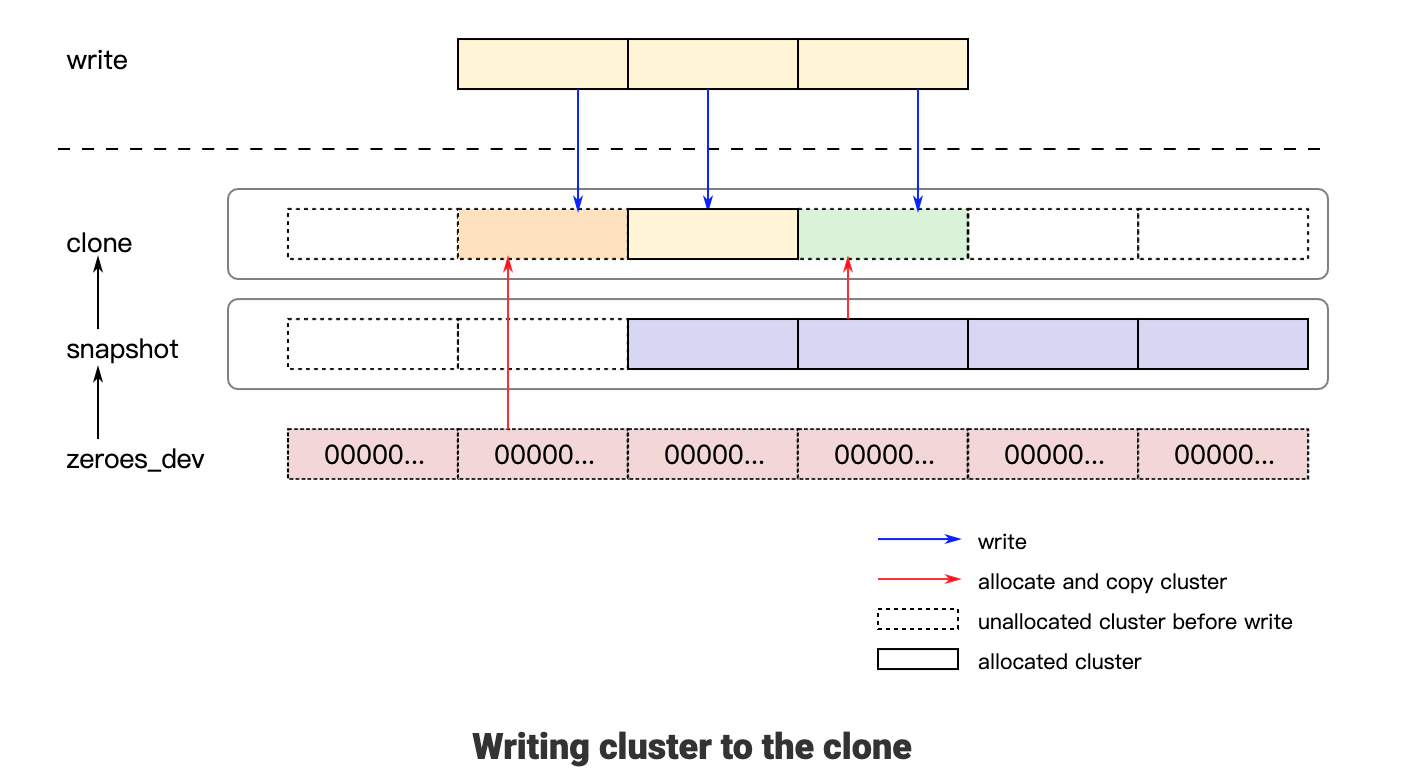
\includegraphics[width=10cm]{../imgs/snapshot/clone-write.png}
\end{center}

\begin{center}
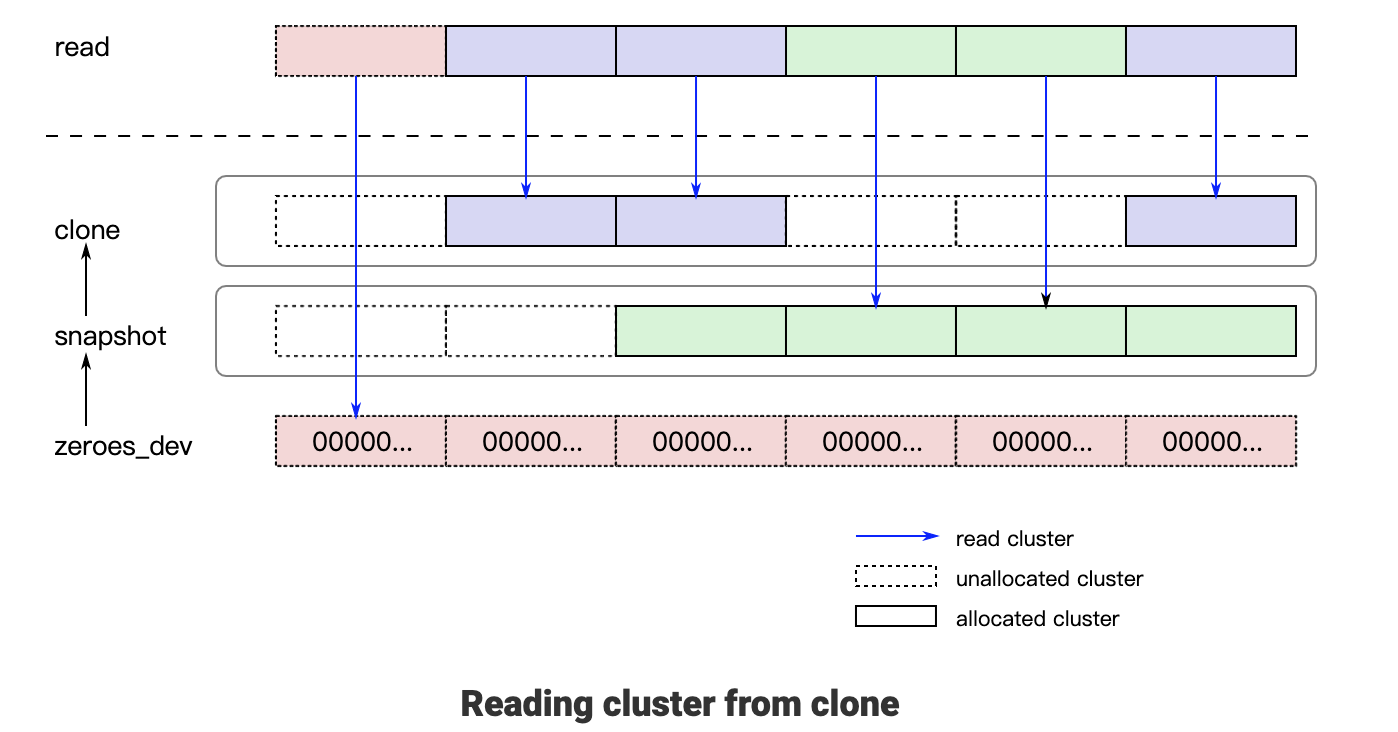
\includegraphics[width=10cm]{../imgs/snapshot/clone-read.png}
\end{center}

\subsection{flatten}

\subsection{protect/unprotect}
